\section{Project Specification}
% The project specification should state clearly what the project is intended to
% deliver, including all hardware, software, simulation, and analytical work, and
% provide some motivation.

\subsection{Project Organisation}
This project is a part of a larger project investigating the effect of using
high radix number systems with on-line arithmetic operators.
The overarching aim would involve implementing such a system on FPGA and
quantifying its performance improvements.
This aim would be achieved through two vertically split individual projects.
One would design and verify the arithmetic operator modules,
while the other would design a system from the top-level to test and
evaluate these operators.
This project deals with the system-level issues.

As this project progresses in parallel with the designing of the operator
modules, it is necessary to decouple the two project so that as individual
projects, they are individually evaluated.
The success of one project should not be restricted by the status of the other.
To this end, the goal of the system-level design is more focussed on its
functionalities and robustness.
This relationship and its effect on the evaluation will be examined further in
the evaluation chapter of this report.

To ensure the two product will work together once they are both complete, a
common interface needs to be agreed upon.
This falls off directly from the use of the hardware and as such it will be
explained in the corresponding section.

% \subsection{Project Interfacing}
% REVISIT: project interfacing section necessary?

\subsection{Deliverables}
At the end of the project, the system should be able to perform the following:
\begin{enumerate}
  \item Takes in the arithmetic modules designed by the sister project as its
        input;
  \item Generate and run tests on these modules;
  \item Vary the frequency and voltage of the FPGA;
  \item Evaluate its performance.
\end{enumerate}

\subsection{Hardware Choice}
The system itself will be built on a Cyclone V SX SoC Development Board from
Intel~\cite{Intel1}.

The 5CSXFC6D6F31C6N SoC has an Arm Cortex-A9 MPCore accompanied by Intel's 28nm
FPGA fabric~\cite{Altera1}.
The FPGA is necessary for implementing the hardware design and obtaining
empirical results for the project.
% maybe hybrid architecture soc makes programming it harder and it could
% be used as a negative point

\begin{figure}[H]
  \centering
  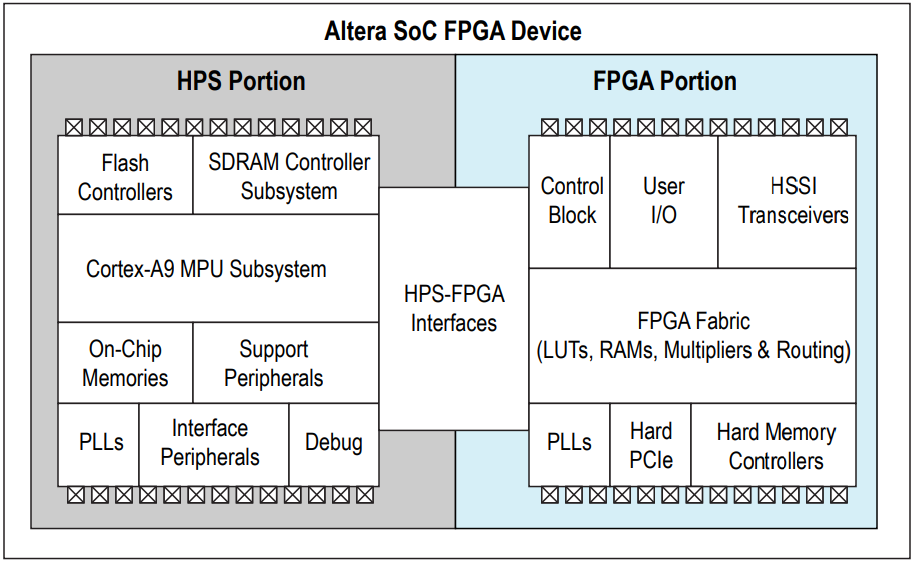
\includegraphics[width=8cm]{img/SoCStructure}
  \caption{Structure of the System-on-Chip}
  \label{SoCStructure}
\end{figure}

While a plain FPGA chip would be enough for this project to work,
having an HPS on the same chip is useful as the test software can run on it.
While allows a better user interface to be constructed with more detailed,
on-the-fly control to the FPGA.
This means to setup the testbench would only require programming in the FPGA
with the design, and running the test script on the HPS.
The product would be self-contained.
It would be more accessible as no additional setup is required for the user.

It should be noted that Xilinx offers similar boards as well.
Its Zynq SoC family has a very comparable structure as they too integrate the
software programmability of an Arm processor with the hardware possibility of
an FPGA.
For example, like the Cyclone V SX, Zynq-7000S also features an Arm Cortex-A9
coupled with a Xilinx 28nm FPGA~\cite{Xilinx1}.
As such, a board like the ZedBoard~\cite{Xilinx2} could be just as viable.

As there are very few significant functional differences between the two brands,
this project will initially explore with the Intel board, simply for its
availability and the personal familiarity with their development tools.

Once the project has progressed to a point where the system design is mature and
tested, the Xilinx alternative could be explored as an extension.

\subsection{Software Choice}
The software choice follows closely with the hardware choice in this project.
To develop for Intel FPGA, Quartus needs to be used.
The version picked is arbitrary as there is not much functional difference
between the versions that would be critical to the project.
As Quartus Prime 16.0 is the version installed in the computers in the
department.
The project will be using the same version for the convenience.
This naturally means the hardware system will be build with the system
integration tool that comes with Quartus -- Qsys.

Other than the hardware design tools, there are some freedom of choice in the
HPS side of the project.
The test will be build with Python, which will be running on an Ubuntu system
that is installed in the HPS.
This choice is made for there are previous unrelated projects on the same
develop board that uses the same configuration, which means a lot of time
could be saved on getting an operating system booting.